\documentclass[aspectratio=169]{beamer}

\graphicspath{{figs/}}

\usepackage{cmap}
\usepackage[T2A]{fontenc}
\usepackage[utf8]{inputenc}
\usepackage[russian]{babel}
\usepackage{amssymb,amsfonts,amsmath}

\usecolortheme{beaver}
\usefonttheme[onlymath]{serif}
\setbeamertemplate{navigation symbols}{}
\setbeamertemplate{footline}{}
\setbeamertemplate{blocks}[rounded=true,shadow=true]
\setbeamerfont{block title}{size=\small}
\setbeamerfont{block body}{size=\small}
\setbeamersize{text margin left=0.5cm,text margin right=0.5cm}

\begin{document}

\begin{frame}{Направление движения по камере и гироскопу}
    \begin{columns}[T]
        \begin{column}{0.52\textwidth}
            \begin{block}{Дано}
                Видео с камеры и показания гироскопа.
            \end{block}
            \begin{block}{Найти}
                Направление движения объекта в каждый момент.
            \end{block}
            \begin{block}{Критерий}
                Минимальная задержка $\tau$ (отставание оценки от реального
                направления) при тряске не больше, чем у оценки по видео.
            \end{block}
            \small
            \textbf{Результат.} Задержка падает с 0,3--0,6~с до 0--0,2~с.\\[0.2em]
            \scriptsize
            На рисунке: пунктир --- опора (сырое измерение, сглаженное без
            сдвига по времени), оранжевый --- только видео, синий --- с гироскопом.
        \end{column}
        \begin{column}{0.48\textwidth}
            \centering
            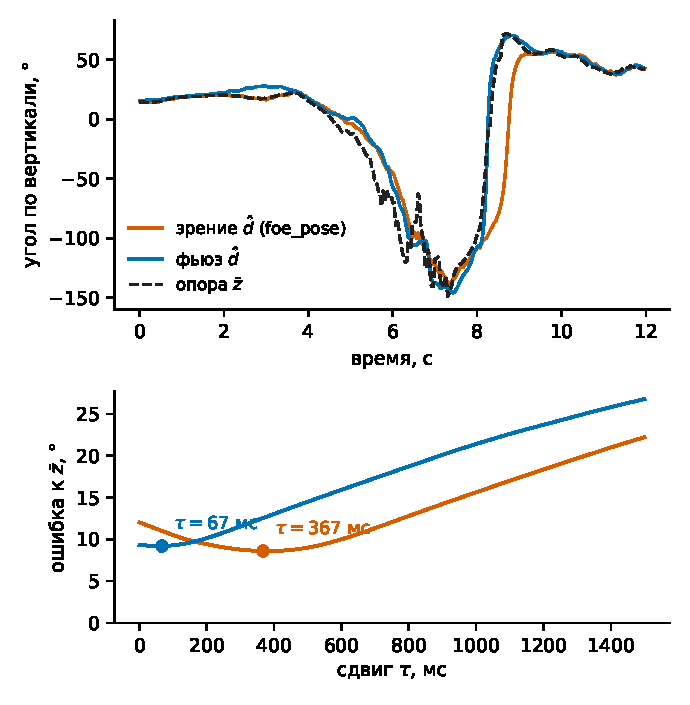
\includegraphics[height=0.70\textheight]{main_figure.pdf}
        \end{column}
    \end{columns}
    \vfill
    \scriptsize
    Задержка, мс (видео $\to$ с гироскопом): окно настройки --- $x$ 333$\to$200, $y$ 367$\to$67;
    проверочное окно --- $x$ 633$\to$0, $y$ 567$\to$133. На проверочном окне отклонение от опоры по $y$ выросло с $9^\circ$ до $18^\circ$.
\end{frame}

\end{document}
